\section{Results and Analysis}\label{sec:results}
All numbers in this section are written by \texttt{code/experiments/aggregate.py} from the result files. Cell-wise values are geometric means over three seeds; intervals are 95\%.

\subsection{Where each family wins, and by how much (the evidence base)}\label{sec:results-study}
\paragraph{Main problems} \Cref{fig:main} shows the outcome $\bar y$ of \eqref{eq:y} for the reduced-basis group against the direct networks. Among the \NMainProblems{} main problems (those with the full budget range), the reduced-basis group is clearly better in \ClsLsAtThirtytwo{} problems at $N=32$, the networks in \ClsNlAtThirtytwo{}, and \ClsTieAtThirtytwo{} are ties; at $N=1024$ the counts are \ClsLsAtTentwentyfour{}, \ClsNlAtTentwentyfour{} and \ClsTieAtTentwentyfour{}. The number of network wins at $N=1024$ is \NlClearTieBandZeroonefive{} if the tie band is widened to 0.15 decade and \NlClearTieBandZerozerofive{} if it is narrowed to 0.05, so counts of ties and small wins are not stable. Where the reduced basis wins, it can win by orders of magnitude (panel b, top rows); where networks win, the largest margin is a factor of about three.
\begin{figure}[t]\centering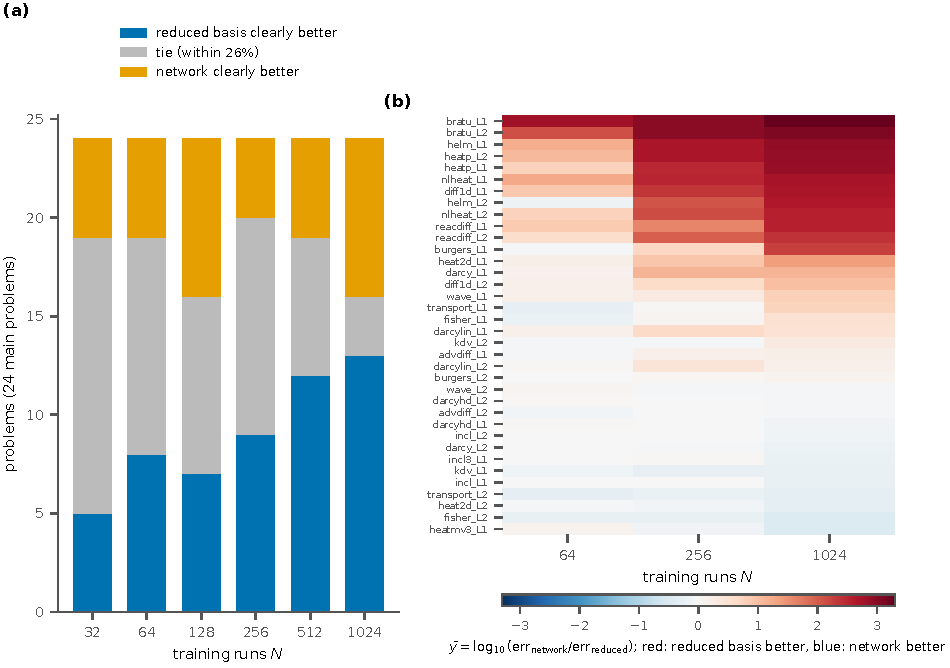
\includegraphics[width=\textwidth]{figures/fig_main_result.pdf}
\caption{The reduced-basis group wins clearly on smooth problems at large budgets, and most differences at small budgets are ties. (a) Number of the \NMainProblems{} main problems (own solvers; five methods; three seeds; tie band $\pm0.1$ decade) in which the reduced-basis group is clearly better, tied, or clearly worse than the direct networks, by training budget. (b) Median signed effect $\bar y$ by problem class over all \NAllProblems{} problems (number of problems in brackets; $\dagger$: solved with \texttt{scikit-fem}); the colour scale is centred at zero and blue is the same colour as in (a). Per-problem values are in Supplement Table~\ref{tab:S-perproblem}. The $N=1024$ results are confounded with a doubling of the networks' optimiser steps (Supplement Sec.~\ref{sec:S-earlier}).}\label{fig:main}\end{figure}
\paragraph{Accuracy reached} For a coarse target of 10\% error, both groups reach it on all 36 own-solver problems within 1024 runs; for 1\% they are about equal (\BudgetLsOne{} against \BudgetNlOne{} problems); at the demanding end, 0.1\%, the reduced-basis group reaches it on \BudgetLsTenth{} problems and the networks on \BudgetNlTenth{} (\BudgetMainLsTenth{} against \BudgetMainNlTenth{} among the 24 main problems, excluding the eight smooth problems we added later because we expected the Gaussian process to do well). On our own problems a solve takes a median of \FomMedianMs{}~ms, so fitting a surrogate costs more than running the simulation 1024 times on most of them; the case for surrogates rests on simulations much slower than ours, and the comparison that matters is accuracy per run.
\paragraph{Problems solved by third-party code (H5)} On the eight problems solved by \texttt{scikit-fem}, the reduced-basis group is clearly better at $N=1024$ in \TpLsClear{} of \TpN{}; the criterion of at least five (H5) is therefore \textbf{\TpVerdict}. The other problems are ties or network wins (Table~\ref{tab:S-perproblem}): the networks are ahead on the composite-conduction problem with nine inputs and high contrast and on both moving-source problems. The simple picture ``reduced basis wins at large budgets'' therefore does not carry over to \TpNotClear{} of these \TpN{} problems; the tool of \cref{sec:method} is designed for exactly this case, and \cref{sec:results-tool} tests it.

\subsection{Why the Gaussian-process reduced model wins when it does}\label{sec:results-mech}
\Cref{fig:mech} compares alternatives with the Gaussian-process reduced model in the \KrrNarrowN{} budget--problem combinations (budgets 64, 256, 1024) where it clearly beats the best network (the comparison uses the best network by \emph{test} error, an oracle that favours the networks). Kernel ridge with the narrow range of ridge and length-scale of our first control is a median \KrrNarrowRatio{} times less accurate; with a wide range and the same eight tuning trials, \KrrWideEightMed{} times; with 32 trials, \KrrWideThirtytwoMed{} times (\KrrWideThirtytwoShare{} of cells within a factor three), and the wide kernel ridge beats the best network clearly in \KrrWideThirtytwoBeat{} of these cells. A Gaussian process on the full field without POD is as accurate as the POD-based one (median ratio \FullOverPod). The Gaussian-process advantage is therefore largely an advantage of a smooth regressor whose regularisation is searched widely and finely, and not of the reduced basis; we did not isolate the contribution of marginal-likelihood fitting, because its cost is not matched by the kernel-ridge search. The wide-range control was added after an AI-agent review of an earlier draft showed that our first control could not reach the regularisation that near-interpolating fits need; this is a post hoc control (Supplement, Sec.~\ref{sec:S-prereg}).
\begin{figure}[t]\centering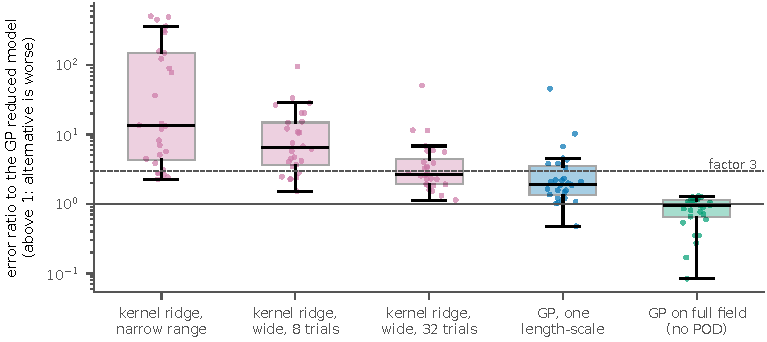
\includegraphics[width=0.85\textwidth]{figures/fig_mechanism.pdf}
\caption{Widening the hyper-parameter search of kernel ridge closes most of the gap to the Gaussian-process reduced model, and a Gaussian process on the full field is as good as the POD-based one. Error ratio of each alternative to the reduced-basis Gaussian process in the \KrrNarrowN{} budget--problem combinations where that model clearly beats the best network (own-solver problems, budgets 64, 256, 1024); boxes show quartiles, dots individual combinations, the dashed line a factor of three.}\label{fig:mech}\end{figure}
Three further results qualify the picture. Training the networks four times longer moved the verdict in \ExpBChanged{} of \ExpBTotal{} cases, always toward the networks, and improved \ExpBImproved{} of the refits; the large gaps survived stronger training (double precision, 6000 steps, L-BFGS) in \ExpFKept{} of \ExpFN{} decisive problems, with the networks' error floor lowered by a median \ExpFGain{} decade to about \NnFloorF. On the extrapolation test set the median $\bar y$ at $N=1024$ is \ExtMedianExt{} instead of \ExtMedianInterp{}. And the class of a cell agrees between halves of the random-search draws in \DrawAgree{} of cases (sign of clear differences: \DrawSign), so small differences should not be over-interpreted. The earlier-stage hypotheses, including the pilot diagnostic that was not confirmed, are in the Supplement (Sec.~\ref{sec:S-earlier}).
